\documentclass[11pt]{amsart}


\usepackage[ibidtracker=false,uniquename=false,giveninits=true,terseinits=true,backend=biber]{biblatex}
\usepackage{float}
\usepackage{graphicx}
\usepackage{todonotes}
\usepackage{subcaption}
\usepackage{amsmath}
\usepackage{amsthm}
\usepackage{amssymb}
\usepackage{algorithm}
\usepackage[noend]{algorithmic}
\usepackage[foot]{amsaddr}
\usepackage[misc]{ifsym}
\usepackage{enumitem}
\usepackage{geometry}
\usepackage[hidelinks]{hyperref}

\renewbibmacro{in:}{}
\addbibresource{rnni_geometry.bib}
\AtEveryBibitem{
	\clearlist{language}
}

\setlist{leftmargin = 0pt}
\geometry{margin=1in}


\newtheorem{proposition}{Proposition}
\newtheorem{theorem}{Theorem}
\newtheorem{lemma}{Lemma}
\newtheorem{corollary}{Corollary}
\newtheorem{problem}{Problem}
\newtheorem{conjecture}{Conjecture}

\newcommand{\lemmaautorefname}{Lemma}
\newcommand{\corollaryautorefname}{Corollary}
\renewcommand{\sectionautorefname}{Section}
\renewcommand{\subsectionautorefname}{Subsection}

\newcommand{\tocite}{ {\color{red}\fbox{CITATION}} }
\newcommand{\toref}{ {\color{blue}\fbox{Reference}} }
\newcommand{\rnni}{\mathrm{RNNI}}
\newcommand{\findpath}{\textsc{FindPath}}
\newcommand{\mrca}{\mathrm{mrca}}
\newcommand{\rank}{\mathrm{rank}}
\newcommand{\ntime}{\mathrm{time}}
\newcommand{\nni}{\mathrm{NNI}}
\newcommand{\spr}{\mathrm{SPR}}
\newcommand{\tbr}{\mathrm{TBR}}
\newcommand{\fp}{\mathrm{FP}}
\newcommand{\dtt}{\mathrm{DtT}}
\newcommand{\np}{\mathbf{NP}}
\newcommand{\decprob}[1]{\rnni(#1)\text{-}\mathrm{SP}}
\newcommand{\rad}{\mathit{rad}}
\renewcommand{\O}{\mathcal O}
\renewcommand{\epsilon}{\varepsilon}
\renewcommand{\thesubfigure}{\Alph{subfigure}}

\newcommand{\algorithmautorefname}{Algorithm}

\newcommand{\summary}[1]{\textbf{#1}} % Print summaries to .pdf
% \newcommand{\summary}[1]{} % Hide summaries in .pdf

\newcommand{\todefine}[1]{{\color{blue}{We need to define:#1}}} % Print summaries to .pdf

\DeclareMathOperator*{\argmin}{argmin}
\DeclareMathOperator*{\argmax}{argmax}

\graphicspath{{figures/}}

\sloppy


\title[Geometry of ranked tree spaces]{The Geometry of the Ranked Nearest Neighbour Interchange Space}
\date{\today}
\author{Lena Collienne}
\email{lcollienne@cs.otago.ac.nz}
\address{Department of Computer Science, University of Otago, New Zealand}
\author{Alex Gavryushkin\textsuperscript{\Letter}}
\email{\textsuperscript{\Letter}alex@biods.org}
\thanks{}

\begin{document}

\begin{abstract}
\end{abstract}

\maketitle


\section{Introduction}

\todo{Include Alex's idea from github issue \#1}
\summary{Why we want time-trees}

\summary{Why discrete time-trees -- Summarising for example}

\summary{How recent results about $\rnni$ make this space interesting and that it is strongly connected to $\dtt_m$}

\summary{Why we want to investigate geometrical properties of $\dtt_m$ and $\rnni$, and also $\rnni(\rho)$}

\summary{Structure of the paper.}


\section{Technical Introduction}

\summary{Introducing discrete time-trees and ranked trees}
A binary rooted phylogenetic tree is a binary tree on a fixed number $n$ of leaves, which are uniquely labelled by elements of the set $\{a_1, \ldots, a_n\}$.
The main objective of study in this paper are \emph{discrete time-trees}, binary rooted phylogenetic trees with positive integer-valued \emph{times} assigned to nodes.
More specifically, all leaves are assigned time $0$, and every internal node is assigned a unique time, such that it always has time greater than its children.
We denote the time of an internal node $v$ by $\ntime(v)$.
If not stated otherwise, we refer to discrete time-trees simply as \emph{trees}.
We furthermore call two trees (not necessarily binary) \emph{identical} if there is a graph isomorphism between them preserving leaf labels and times.
The number of discrete time-trees with root time less or equal to $m$ is $\frac{(n-1)!n!m^{n-1}}{2^{n-1}}$ \autocite{Gavryushkin2018-ol}.

As special case of discrete time-trees we consider \emph{ranked trees} with root time $n-1$.
In these trees internal nodes are uniquely labelled by times in $\{1, \ldots, n-1\}$.
This definition of ranked trees coincides with the one of \textcite{Collienne2020-iu}.
In the case of ranked trees we say \emph{rank} of a node $v$ to mean its time ($\rank(v) = \ntime(v)$) to be consistent with notations used in \autocite{Collienne2020-iu}.

Every internal node $v$ of a tree $T$ can be referred to by the set $C$ of leaves that are descending from this node.
We call such a set $C$ \emph{cluster} and say that the cluster $C$ is \emph{induced} by $v$.
A list of clusters $[C_1, \ldots, C_{n-1}]$ uniquely defines a ranked tree, where cluster $C_i$ is induced by the internal node with rank $i$ for $i \in \{1, \ldots, n-1\}$.
For discrete time-trees however, times of nodes also need to be provided to uniquely identify a tree.
For a subset $S \subseteq \{a_1, \ldots, a_n\}$ we call the internal node of a tree $T$ with lowest time among those ancestral to all elements of $S$ the \emph{most recent common ancestor} of $S$ and denote it by $(S)_T$.
We furthermore denote the parent of a leaf $a_i$ in $T$ by $(a_i)_T$, and the cluster induced by the node with time $i$ in $T$ by $(T)_i$.
An important type of trees that will be of importance throughout the whole paper are \emph{caterpillar trees}, which are trees where every internal nodes has at least one child that is a leaf.

\summary{Defining the tree space $\dtt_m$ and $\rnni = \dtt_{n-1}$}
We are now ready to introduce the central object of study of this paper, the graph (or space) of discrete time-trees.
This graph is called $\dtt_m$ for a fixed positive integer $m$.
The vertex set of $\dtt_m$ is the set of trees with root time less or equal to $m$.
Trees $T$ and $R$ are connected by an edge ($T$ and $R$ are \emph{neighbours}) in this graph if performing one of the following (reversible) operations on $T$ results in $R$:
\begin{enumerate}
	\item An \emph{$\nni$ move} connects trees $T$ and $R$ if there is an edge $e$ in $T$ and an edge $f$ in $R$, both of length one, such that shrinking $e$ and $f$ to nodes results in identical trees.
	\item A \emph{rank move} on $T$ exchanges the times of two internal nodes with time difference one.
	\item A \emph{length move} on $T$ changes the time of an internal node by one.
\end{enumerate}
A length move can only change the time of a node to become $t$ if there is no node with time $t$ already.
Note that our definition of $\dtt_m$ differs from the definition of \textcite{Gavryushkin2018-ol}, as length move are defined differently in their paper.

The definition of $\dtt_m$ leads to a natural definition of the \emph{distance} between two trees $T$ and $R$ in this graph as the length of a shortest paths between these trees, denoted by $d(T,R)$.
We also consider the ranked nearest neighbour interchange ($\rnni$) graph of \textcite{Collienne2020-iu}, which is the graph $\dtt_m$ for $m=n-1$, and hence a graph of ranked trees.
In this graph length moves are not possible, so we use the notion $\rnni$ \emph{move} to mean either a rank move or an $\nni$ move in order to distinguish these moves from length moves.

\todefine{
	\begin{itemize}
		\item $(T)_i$ for cluster induced by node of rank $i$ in $T$ -- this is only needed for proofs around $\rnni(\rho)$ and in the proof that every tree is connected to a caterpillar tree in $\rnni$ by a sequence of $\nni$ moves AND $\findpath$ pseudo-code (!)
		\item We sometimes say $\rnni$ instead of $\rnni$ space. If we keep that, we might want to mention that we do it? -- We use just '$\rnni$' in polynomial paper as well!
		\item distinguish the shortest path problem from the distance problem! -- maybe mention that $\findpath$ is optimal algorithm for shortest path problem
	\end{itemize}
}


\section{Computing Shortest Paths in $\dtt_m$}
\label{section:fp_dtt}

\summary{Introduce how we can use $\findpath$ to compute $\dtt_m$ distances}
Shortest paths, and therefore distances, between trees in $\rnni$ can be computed in quadratic running time with the algorithm $\findpath$, introduced by \textcite{Collienne2020-iu}.
As $\rnni$ is a special case of $\dtt_m$ for $m = n-1$, the question whether this algorithm can also be used to compute shortest paths in $\dtt_m$ arises.
In this section we present a generalisation of $\findpath$ that computes distances between trees in $\dtt_m$.
Before introducing the version of $\findpath$ for $\dtt_m$, we introduce a way to convert trees in $\dtt_m$ into ranked trees, such that the $\rnni$ distance between those ranked trees equals their distance in $\dtt_m$ (\autoref{thm:dtt_findpath}).

\summary{How to add leaves to a $\dtt_m$ tree to transform it into a ranked tree}
A tree $T$ in $\dtt_m$ can be converted into a ranked tree in $\rnni$ on $m+2$ in the following way (\autoref{alg:ranked_tree}).
First add a new root with time $m + 1$ that becomes parent of the root of $T$.
The second child of this new root is the root of a caterpillar tree on leaf set $\{a_{n+1}, a_{n+2}, \ldots, a_{m+2}\}$, such that $\ntime(a_{n+1}) = \ntime(a_{n+2}) < \ntime(a_{n+3}) < \ldots < \ntime(a_{m+2})$.
The resulting tree $T_r$ is hence a uniquely defined ranked tree with $m+2$ leaves.
An example of this extension of a tree $T$ to a ranked tree $T_r$ is depicted in \autoref{fig:dtt_to_ranked_tree}.

Throughout this paper we use the index $r$ for $T_r$ to refer to this extended ranked version of a tree $T$.
Moreover, we denote the subtree of $T_r$ that is identical to $T$ by $T_r^d$ ($d$ for discrete time-tree) and the caterpillar subtree on leaf set $\{a_{n+1}, \ldots, a_{m+2}\}$ by $T_r^c$.

\begin{algorithm}[ht]
	\caption{RankedTree($T$, $m$)}
	\label{alg:ranked_tree}
	\begin{algorithmic}[1]
		\STATE $S:= \{1 \leq i \leq m | \text{ no internal node in } T \text{ has time } i\}$
		\STATE $[i_1, \ldots, i_{m-n+1}] = sort(S)$
		\STATE $T_r^d =$ copy of $T$
		\STATE $T_r^c =$ tree consisting of just one internal node $v_1$ with rank $i_1$ and children $a_{n+1}, a_{n+2}$
		\FOR {$k = 2, \dots, m-n+1$}
			\STATE Add internal node $v_k$ with with time $i_k$ and children $v_{k-1}$ and $a_{n+1+k}$ to $T_r^c$
		\STATE $T_r = $ tree with root with time $m+1$ and children of root are roots of $T_r^d$ and $T_r^c$.
		\ENDFOR
		\RETURN $T_r$
	\end{algorithmic}
\end{algorithm}

\begin{figure}[ht]
	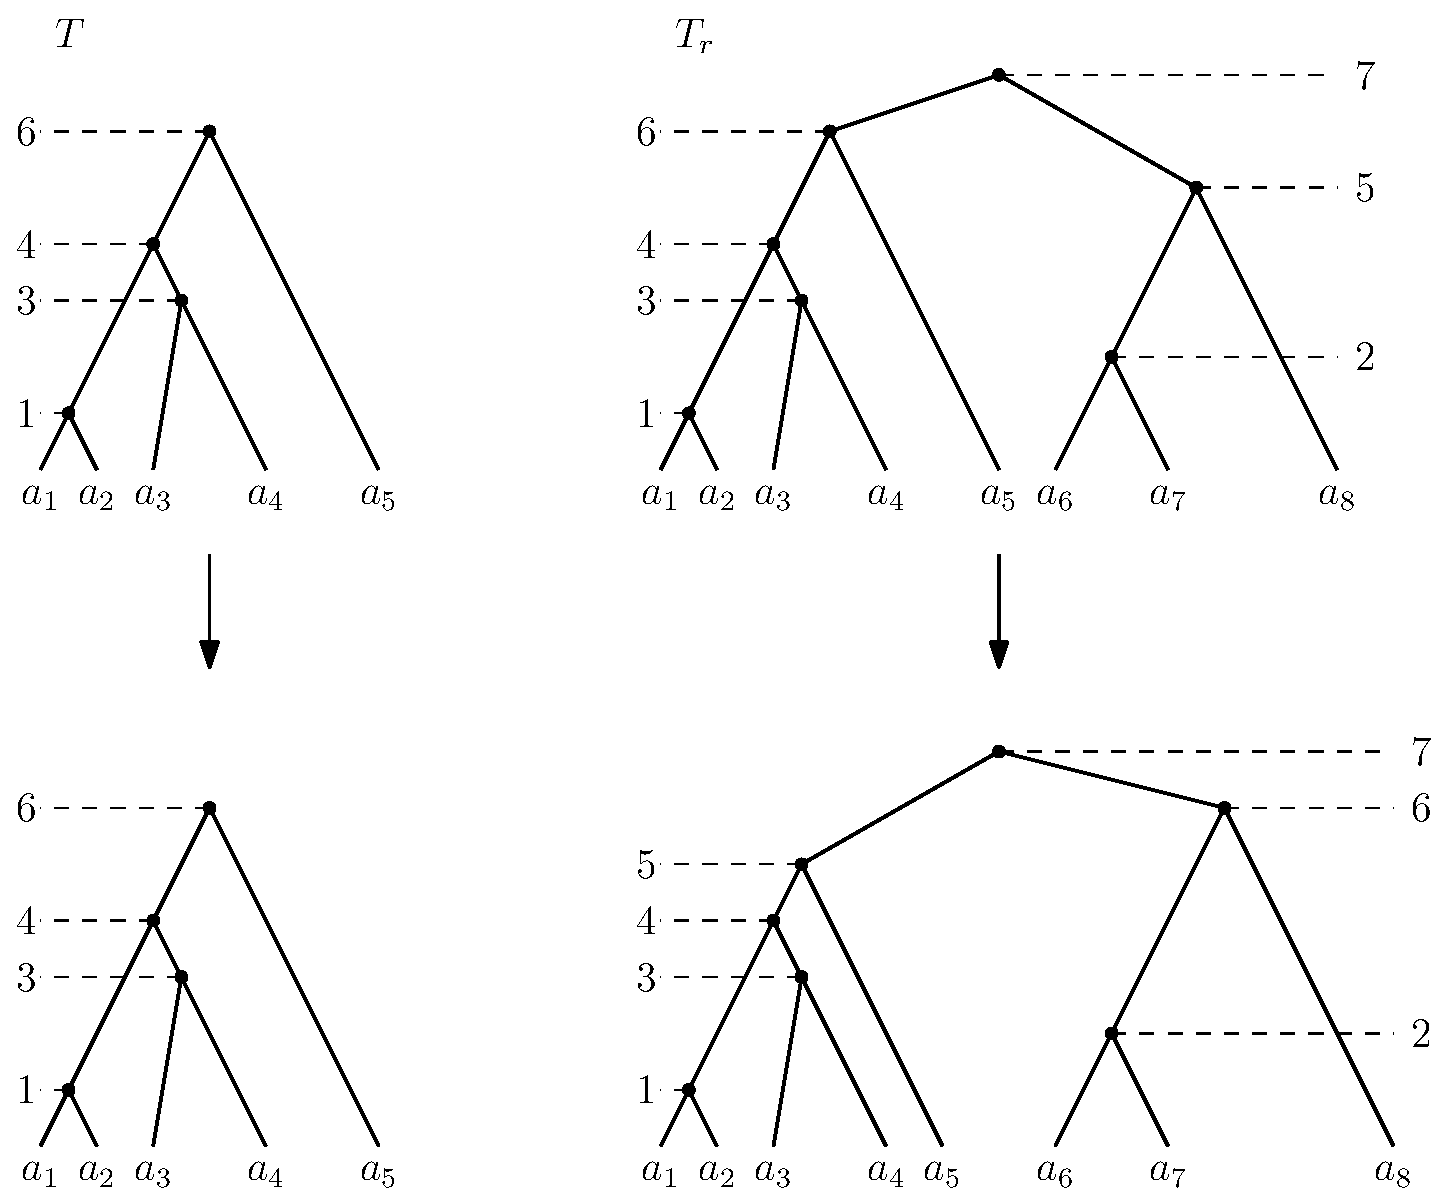
\includegraphics[width=0.75\textwidth]{dtt_to_ranked_tree.eps}
	\caption{Extending a tree $T$ on $n$ leaves in $\dtt_6$ (top left) to a ranked tree with $m+2=8$ leaves (top right) by adding a caterpillar subtree with three leaves.
	The trees on the bottom result from $T$ and $T_r$ by performing a length move (left) or rank move (right), respectively).}
	\label{fig:dtt_to_ranked_tree}
\end{figure}

\summary{Moves on the extended ranked versions of trees -- $\rnni$ vs length moves}
In the following we distinguish not only rank moves and $\nni$ moves on the extended ranked version $T_r$ of a tree $T$, but we will also distinguish two different types of rank moves.
Rank moves between one node of $T_r^c$ and one node of $T_r^d$ can be interpreted as length moves in $T_r^d$ (\autoref{fig:dtt_to_ranked_tree}).
Therefore, we will refer to such rank moves as \emph{rank moves corresponding to length moves}.
All remaining rank moves will still be called rank moves.
Note that the correspondence of rank moves between $T_r^c$ and $T_r^d$ to length moves in $T$ shows that any path between $T$ and $R$ in $\dtt_m$ can be interpreted as a path between $T_r$ and $R_r$ in $\rnni$.

\summary{How to compute shortest $\dtt_m$-paths between trees with $\findpath$}
After extending both trees $T$ and $R$ in $\dtt_m$ to ranked trees $T_r$ and $R_r$ on $m+2$ leaves, respectively, we can compute shortest paths between $T_r$ and $R_r$ in $\rnni$, using $\findpath$.
A path computed by $\findpath$ preserves clusters \autocite{Collienne2020-iu}, hence there are no $\nni$ moves in the newly added caterpillar subtree on the leaf set $\{a_{n+1}, \ldots, a_{m+2}\}$ on such a path.
The only moves involving internal nodes of this caterpillar subtree are rank moves that correspond to length moves, as described above.
Hence the path $\fp(T_r,R_r)$ provides a path between $T$ and $R$ in $\dtt_m$, when only considering the subtrees induced by $\{a_1, \ldots, a_n\}$ in all trees on $\fp(T_r, R_r)$, interpreting some rank moves between $T_r$ and $R_r$ as length moves.
We denote this path in $\dtt_m$, which results from $\fp(T_r, R_r)$, by $\fp(T,R)$.
In \autoref{thm:dtt_findpath} we establish that $\fp(T,R)$ is a shortest path in $\dtt_m$ indeed.
Note that for any given pair of trees $T$ and $R$, if not specified otherwise, we always assume $m$ to be the maximum root time of these trees in and aim to compute a shortest path between them in $\dtt_m$. 

\begin{theorem}
	The path $\fp(T,R)$ between two discrete time-trees $T$ and $R$ is a shortest path in $\dtt_m$, where $m$ is the maximum root time of $T$ and $R$.
	\label{thm:dtt_findpath}
\end{theorem}

\begin{proof}
	Let $T$ and $R$ be discrete time-trees and $T_r$ and $R_r$ their extended ranked versions computed with \autoref{alg:ranked_tree}, respectively.
	Any path in $\dtt_m$ from $T$ to $R$ gives a path of equal length between $T_r$ and $R_r$ in the $\rnni$ space on $m+2$ leaves.
	This is due to the fact that the only moves needed in the subtree $T_r^c$ to transform it to $R_r^c$ are rank moves that correspond to length moves, and no other $\rnni$ moves.
	If there was a path between $T$ and $R$ shorter than $\fp(T,R)$, the corresponding path between $T_r$ and $R_r$ in $\rnni$ would be shorter than the one computed by $\findpath$ in this space.
	Since this contradicts \autocite[Theorem 1]{Collienne2020-iu}, it follows that $\fp(T,R)$ is a shortest path in $\dtt_m$.
\end{proof}

\summary{Running time of $\findpath$ + we don't need to add subtree in practice}
\autoref{thm:dtt_findpath} shows that $\findpath$ (\autoref{alg:fp_dtt}) computes shortest path between two trees in $\dtt_m$ in polynomial time, more specifically in $\O(mn)$.
More details on this are provided in \autoref{section:diameter} following \autoref{thm:dtt_diameter}.
It is not even necessary to convert a given pair of discrete time-trees to ranked trees to apply $\findpath$ to them.
Instead, we modify $\findpath$ for trees in $\dtt_m$.
Iterations of $\findpath$ that consider clusters in the added caterpillar trees are replaced by length moves increasing the time of internal nodes as described in the \textbf{for} loop in Line~\ref{line:length_move} of \autoref{alg:fp_dtt}.
The benefit of this modified version of the algorithm, compared to using $\findpath$ on the extended ranked versions of the trees, is a reduced use of memory, which is especially of practical relevance for $m >> n$.

\begin{algorithm}[h]
	\caption{$\findpath$($T,R$)}
	\begin{algorithmic}[1]
		\label{alg:fp_dtt}
		\STATE $T_1 := T$, $p := [T_1]$
		\FOR {$k = 1, \dots, m$}
			\IF {$R$ has a node with rank $i$}
			\STATE $C:=(R)_i$
			\WHILE {$\rank((C)_{T_1})>k$}
					\STATE $T_2$ is $T_1$ with the rank of $(C)_{T_1}$ decreased by an $\rnni$ move
				\STATE $T_1 = T_2$
				\STATE $p = p+T_1$
			\ENDWHILE
			\ELSE
				\STATE $i := \min\{l | l>k \text{ and no node in } T_1 \text{ has time }l\}$
				\FOR {$j = i-1, \dots, k$}
					\label{line:length_move}
					\STATE $T_2$ is $T_1$ where the time of $(T_1)_j$ is increased by one (length move)
					\STATE $T_1 = T_2$
					\STATE $p = p+T_1$
				\ENDFOR
			\ENDIF
		\ENDFOR
		\RETURN $p$
	\end{algorithmic}
\end{algorithm}


\section{Geometrical Properties of $\dtt_m$}

\subsection{Cluster Property}
\summary{Definition of Cluster Property and why it is relevant (a bit of bio).}
In this section we consider a property of tree spaces.
A tree space has the \emph{cluster property}, if all trees on every shortest paths between two trees sharing a cluster $C$ also contain this cluster.
This is desirable biological property as trees sharing a cluster or subtree are expected to be closer to each other than to a tree not sharing a cluster with them.
An example for the practical relevance of this property are summary trees.
For a given sample of trees containing a common subtree, it is expected that their summary or mean tree also contains this subtree.
It hence is desirable to have a tree space that has the cluster property.

\summary{Cluster property in $\nni$ and its connection to the complexity result.}
A further reason for investigating the cluster property in $\rnni$ is the importance of it in a similar and well studied \tocite tree space, $\nni$.
In the $\nni$ graph trees have no times and $\nni$ moves are allowed on every edge.
Computing distances in $\nni$ is $\np$-hard\autocite{Dasgupta2000-xa}, and the proof relies on the fact that this tree space does not have the cluster property \autocite{Li1996-zw}.
In the $\rnni$ graph, however, distances can be computed in polynomial time by $\findpath$ \autocite{Collienne2020-iu}, which preserves common clusters.
The question whether $\rnni$ has the cluster property is hence natural, and will be settled in \autoref{thm:cluster_property_rnni}.
Note that even though it seems like distances can be computed in polynomial time in a tree space if it has the cluster property, this does not need to be true in general.

\summary{$\rnni$ has the cluster property.}
\begin{theorem}
	The $\rnni$ graph has the cluster property.
	\label{thm:cluster_property_rnni}
\end{theorem}

\begin{proof}
	We assume to the contrary that there are two ranked trees $T$ and $R$ are sharing a cluster $C$, such that there is a path $p$ between these trees where $C$ is not present in every tree on $p$.
	We furthermore assume that there is no pair of trees with a shortest path not containing a shared cluster and distance less than $d(T,R)$, meaning that $T$ and $R$ give a minimum counterexample.
	Because of this minimality assumption on the length of $p$, the first tree $T'$ following $T$ on $p$ does not contain $C$.
	Since only the one cluster $C$ changes by the $\nni$ move between $T$ and $T'$, all nodes with rank below $(C)_T$ induce the same clusters in $T$ and $T'$.
	We now compare distances $d(T,R)$ and $d(T',R)$ by using properties of $\findpath$.

	First we compare $\fp(R,T)$ and $\fp(R,T')$.
	All trees on on these two paths coincide until the point is reached where the cluster considered on $\fp(R,T)$ is $C$.
	Let $R'$ denote the tree at this point of the path.
	Then $\fp(R,T)$ and $\fp(R,T')$ coincide up to this tree $R'$.
	It follows $d(T,R) = d(R,R') + d(R', T)$ and $d(T',R) = d(R,R') + d(R', T')$.

	Now consider $\fp(T', R')$ to evaluate $d(R', T')$.
	As $\findpath$ preserves clusters, $C$ is present in every tree on $\fp(T,R)$ up to and including $R'$.
	The fist iteration of $\findpath$ applied to the pair of trees $(T',R')$ considers the cluster $C$, as all cluster induced by nodes below $(C)_{T'}$ coincide in $R'$ and $T'$.
	To construct the cluster $C$ in $T'$, there is just one $\nni$ move needed, which results in the tree $T$, as $T$ and $T'$ are $\nni$ neighbours such that $T$ contains $C$ and $T'$ does not (\autoref{fig:cluster_property_rnni}).
	We can therefore conclude that $d(T,R) = d(T',R) - 1$, which contradicts the assumption that $T'$ is the first tree on a shortest path from $T$ to $R$.
	There is hence no shortest path between $T$ and $R$ that does not preserve $C$, which proves the cluster property for $\rnni$.
\end{proof}

The fact that a slightly modified version of $\findpath$ computes shortest paths $\dtt_m$ already suggest that shortest path in $\rnni$ and $\dtt_m$ have similar properties.
The cluster property in $\dtt_m$ follows from \autoref{thm:cluster_property_rnni}, indeed.

\begin{corollary}
	The graph $\dtt_m$ has the cluster property.
\end{corollary}

\begin{proof}
	If there was a shortest path between two trees $T$ and $R$ in $\dtt_m$ that did not preserve a common cluster, this path can be seen as a path between $T_r$ and $R_r$, the extended ranked versions of $T$ and $R$ in $\rnni$, as already discussed in \autoref{thm:dtt_findpath}.
	Since this path has the same length as the one between $T_r$ and $R_r$, it is a shortest path in $\rnni$ as well, which leads to a contradiction to \autoref{thm:cluster_property_rnni}.
\end{proof}

\subsection{Caterpillar Trees}

\summary{Defining Caterpillar trees. Why are they interesting?}
In this subsection we focus on the set of caterpillar trees and establish some properties of shortest paths between those trees in both $\rnni$ and $\dtt_m$.
A path between two caterpillar trees only consisting of caterpillar trees is a \emph{caterpillar path}.
In \autoref{thm:caterpillar_convex_dtt} and \autoref{cor:caterpillar_convex_rnni} we will see that, in both $\dtt_m$ and $\rnni$, any two caterpillar trees are connected by a shortest path that is a caterpillar path.
We say that a set of trees for which such a shortest path that stays within this set exists is \emph{convex} in the corresponding tree space.
This is another property of $\rnni$ that the $\nni$ space of unranked trees does not have \autocite{Gavryushkin2018-ol}.
Based on the convexity of the set of caterpillar trees in $\rnni$ we introduce a way to compute distances between caterpillar trees in this space in time $\O(n\log n)$ in \autoref{cor:caterpillar_distance_rnni_nlogn}, and hence with better worst-case time complexity than $\findpath$.

\begin{theorem}
	The set of caterpillar trees is convex in $\dtt_m$.
	\label{thm:caterpillar_convex_dtt}
\end{theorem}

\todo{Check this proof carefully!}
\begin{proof}
	Let $T$ and $R$ be two caterpillar trees in $\dtt_m$.
	We prove the theorem by showing that there is a caterpillar tree $T'$ that is neighbour of $T$ and closer to $R$ than $T$.
	The existence of a shortest path consisting only of caterpillar trees between $T$ and $R$ follows inductively.
	Throughout this proof we consider the extended ranked versions $T_r$ and $R_r$ of $T$ and $R$.

	Let $a_k := \argmax_{a_1, \ldots, a_n}\{\rank(a_i)_{R_r} | \rank(a_i)_{R_r} \neq \rank(a_i)_{T_r}\}$ be the leaf with parent with maximum rank in $R_r$ among those that are not in the same position in $T_r$ and $R_r$.
	Let furthermore $a_j \in \{a_1, \ldots, a_{m+2}\}$ be a leaf with $\rank(a_j)_{T_r} = \rank(a_k)_{T_r} + 1$.
	We define $T'_r$ to be the caterpillar tree resulting from $T_r$ by an $\nni$ move or rank move exchanging the ranks of $(a_k)_{T_r}$ and $(a_j)_{T_r}$.
	An $\nni$ move is necessary if these two nodes are connected by an edge, otherwise a rank move corresponding to a length move is performed on $T_r$ to receive $T'_r$.
	In both cases $T'_r$ is a caterpillar tree.
	By using properties of shortest paths computed by $\findpath$, we now show that $|\fp(R_r,T'_r)| = |\fp(R_r,T_r)| - 1$.

	\todo{update this figure to $\dtt_m$}
	\begin{figure}[ht]
		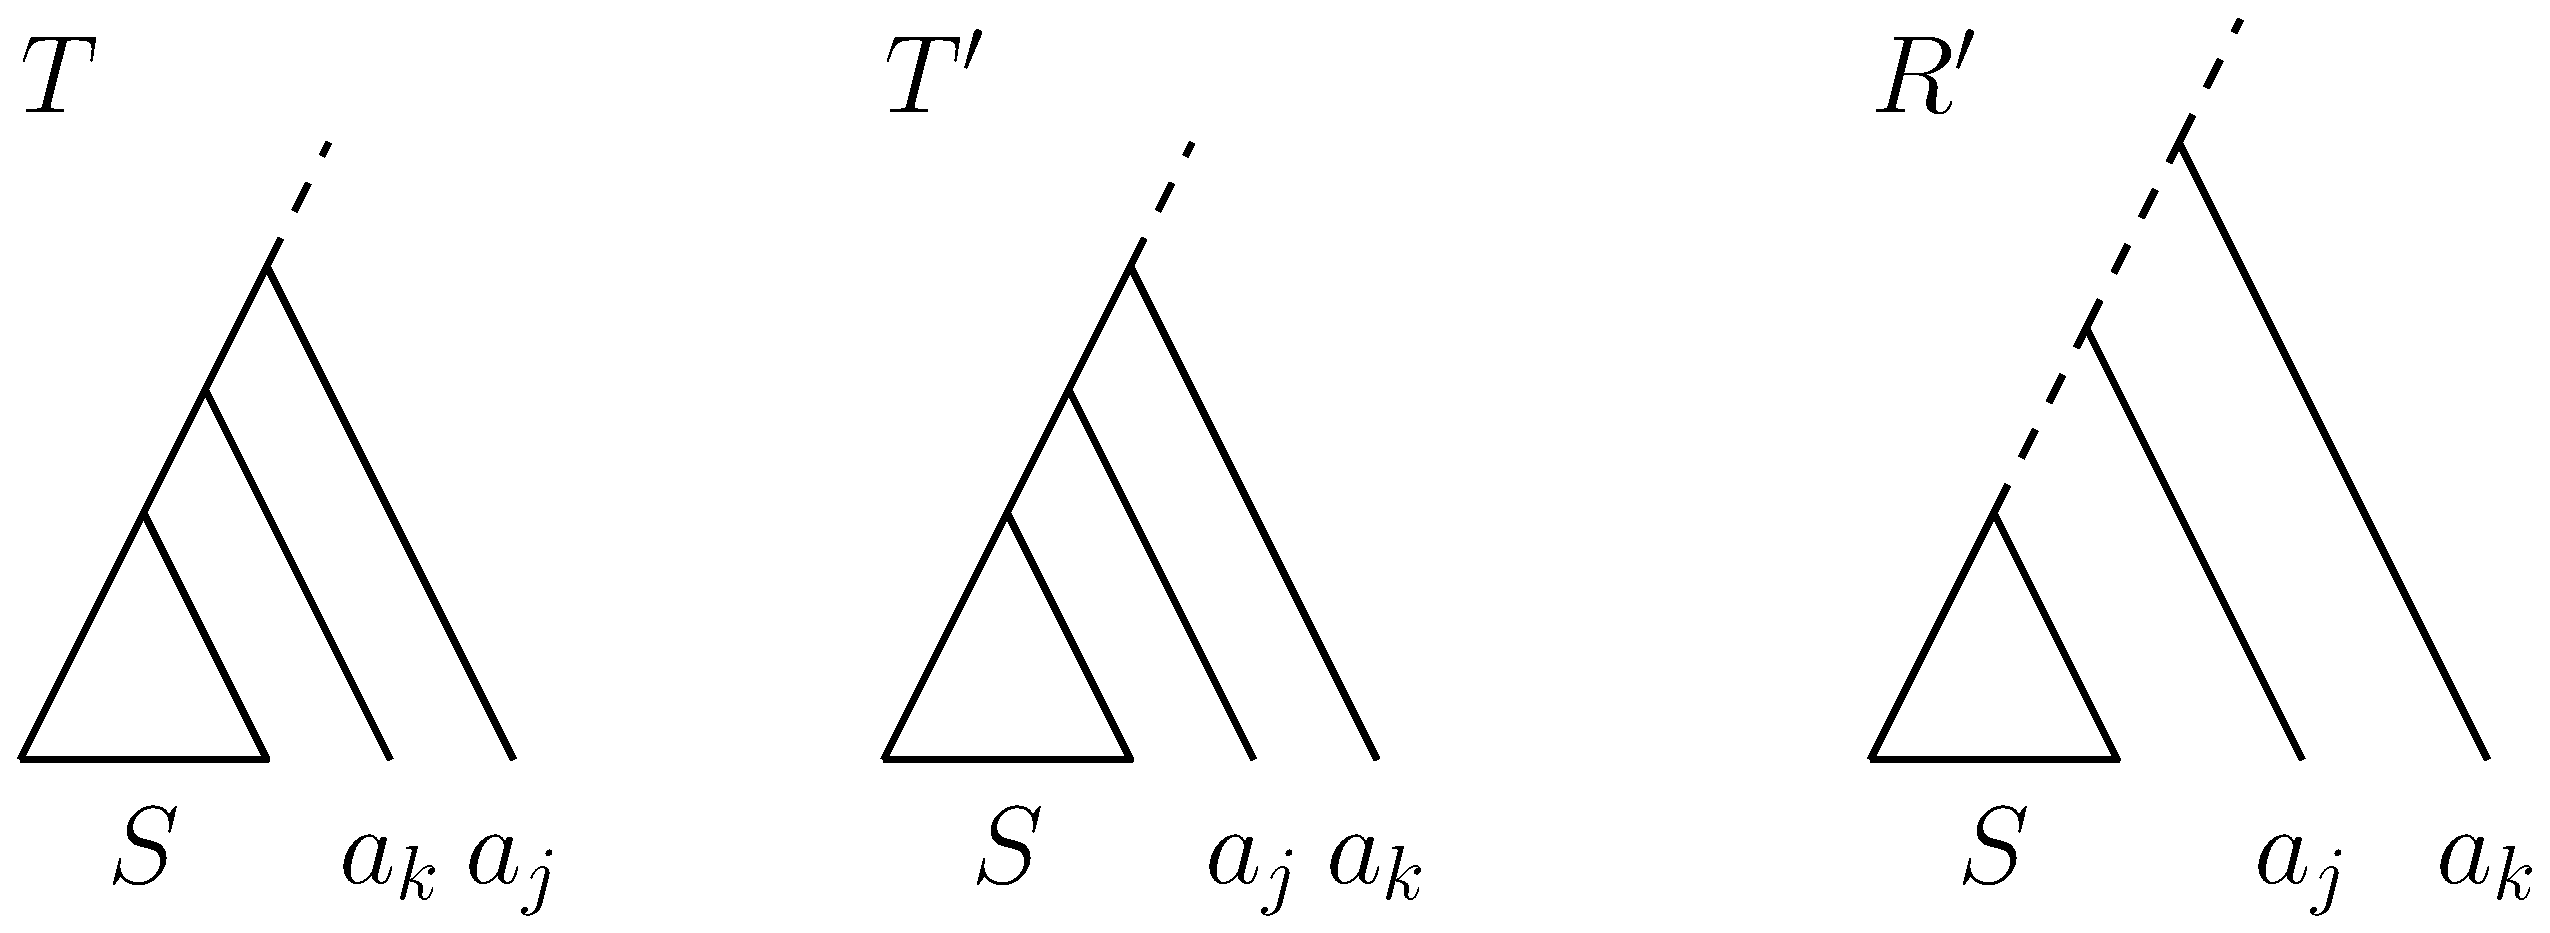
\includegraphics[width=0.66\textwidth]{proof_caterpillar_convex_rnni.eps}
		\caption{Trees $T$, $T'$, and $R'$ as described in the proof of \autoref{thm:caterpillar_convex_dtt}.
		All three trees share the subtree induced by subset $S$ of leaves.
		Between $T$ and $T'$ only leaves $a_j$ and $a_k$ are exchanged.
		Dashed lines represent remaining part of trees, which are equal in $T$ and $T'$.}
		\label{fig:proof_caterpillar_convex_rnni}
	\end{figure}

	Since all clusters of $T_r$ and $T'_r$ induced by nodes of rank less than $\rank(a_k)_{T_r}$ coincide, the paths $\fp(R_r,T_r)$ and $\fp(R_r,T'_r)$ coincide up to a ranked tree $R'_r$, which contains all these clusters.
	We now compare the lengths of $\fp(R'_r,T_r)$ and $\fp(R'_r,T'_r)$.
	Therefore, we note at first that it is $\rank(a_j)_{R_r} < \rank(a_k)_{R_r}$ by the choice of $a_k$, and therefore also $\rank(a_j)_{R'_r} < \rank(a_k)_{R'_r}$.

	By our assumptions on $T_r$, the clusters considered on $\fp(R_r,T_r)$ in the two iterations following $R'_r$ are first $S \cup \{a_k\}$ and then $S' \cup \{a_j\}$ for some clusters $S$ and $S'$ that are present in $T_r$, $T'_r$, and $R'_r$.
	Decreasing the rank of $(S \cup \{a_k\})_{R'_r}$ takes $\rank(S \cup \{a_k\})_{R'_r} - (\rank(S)_{R'_r} + 1)$ $\rnni$ moves.
	Because the rank of $(S \cup \{a_j\})_{R'_r}$ increases by one when the parents of $a_k$ and $a_j$ swap ranks in this iteration, the following iteration for $S' \cup \{a_j\}$ needs $\rank(S' \cup \{a_j\})_{R'_r} + 1 - (\rank(S')_{R'_r} + 2)$ $\rnni$ moves.
	On $\fp(R_r,T'_r)$ however, first $\rank(S' \cup \{a_j\})_{R'_r} - (\rank(S')_{R'} + 1)$ $\rnni$ moves decrease the rank of $(S' \cup \{a_j\})_{R'}$, and then $\rank(S \cup \{a_k\})_{R'_r} - (\rank(S)_{R'_r} + 2)$ are needed for $S \cup \{a_k\}$.
	In total, for both iterations one more move is needed on $\fp(R_r, T'_r)$ compared to $\fp(R_r, T_r)$. 

	The only difference in hte trees after these two iterations on the two different paths is the order of ranks of the parents of $a_j$ and $a_k$.
	Since the rest of $T_r$ and $T'_r$ coincide, the remaining parts of $\fp(R_r, T_r)$ and $\fp(R_r, T'_r)$ consist on the same moves.
	With our previous observation we can conclude $d(R_r,T_r) = d(R_r,T'_r) + 1$, and hence $T'_r$ is on a shortest path from $T_r$ to $R_r$.
\end{proof}

The convexity of the set of caterpillar trees in $\rnni$ follows from the convexity of this set in $\dtt_m$ for $m = n-1$ (\autoref{thm:caterpillar_convex_dtt}).

\begin{corollary}
	The set of caterpillar trees is convex in $\dtt_m$.
	\label{cor:caterpillar_convex_rnni}
\end{corollary}

\summary{With Theorem~\ref{cor:caterpillar_convex_rnni} we can find a more efficient way to compute distances between caterpillar trees.}
Using the convexity of the set of caterpillar trees (\autoref{thm:caterpillar_convex_dtt}) in $\rnni$, there are several algorithms of computing the distance between two caterpillar trees.

A problem analogous to the shortest path problem for caterpillar trees is the \emph{Token Swapping Problem} (TSP) \autocite{Kawahara2017-ey} on a special class of graphs, so-called lollipop graphs.
The only moves possible between caterpillar trees are $\nni$ moves, which simply swap two leaves, and these can be translated to swapping two tokens in TSP.
\textcite{Kawahara2017-ey} provide an algorithm for TSP on lollipop graphs, which can be used for computing distances between caterpillar trees in $\rnni$ as well.
This algorithm however has worst-case time complexity $\O(n^2)$, the same as $\findpath$.

We are however able to present an algorithm with better worst-case complexity, specifically in $\O(n \log n)$ for $\rnni$ (\autoref{cor:caterpillar_distance_rnni_nlogn}).
Therefore, we first present in \autoref{thm:caterpillar_distance_formula} a formula to express distances between two caterpillar trees in $\rnni$.

\begin{theorem}
	Let $T$ and $R$ be caterpillar trees in $\rnni$ such that \[1 = \rank(a_1)_R = \rank(a_2)_R < \rank(a_3)_R < \ldots < \rank(a_n)_R = n-1\]
	and
	\[P_T := \{(i,j)| \rank(a_i)_T < \rank(a_j)_T \text{ and } \rank(a_i)_R > \rank(a_j)_R\},\]
	\begin{align*}
		M_T := &\{a_i| (\forall l \textnormal{ with } \rank(a_l)_T \leq \rank(a_i)_T: \rank(a_l)_R > \rank(a_i)_r)\} \\
		& \cap \{a_i | \rank(a_i)_T < \min\{\rank(a_1)_T, \rank(a_2)_T\}\}
	\end{align*}
	Then it is
	\[d(T,R) = p_T - m_T,\]
	for ${m_T = |M_T|}$ and ${p_T = |P_T|}$.
	\label{thm:caterpillar_distance_formula}
\end{theorem}

We refer to pairs $(i,j) \in P_T$, as defined in \autoref{thm:caterpillar_distance_formula}, as transpositions.
The reason for this is that the caterpillar trees can be seen as permutations of the set $\{a_1, \ldots, a_n\}$, ordered according to increasing rank of their parents.
The tree $R$ then corresponds to the identity permutation $(a_1, a_2, a_3, \ldots, a_n)$.
We therefore call elements in $P_T$ transpositions.
Note that there is no one-to-one correspondence between permutations and caterpillar trees.
For example the permutation $(a_2, a_1, a_3, \ldots, a_n)$ corresponds to the tree $R$ as well, as the first two elements share a parent in the caterpillar tree.
Therefore, the two pairs that share parents in $T$ and $R$, respectively, are not in the set $P_T$.

\begin{proof}
	Let $T$ and $R$ be caterpillar trees as described above and $\hat d(T,R) = p_T - m_T$.
	For proving $\hat d(T,R) = d(T,R)$, it is sufficient to show that for all caterpillar trees $T'$ that are neighbour of $T$ it is
	\begin{align}
		\hat d(T',R) \geq \hat d(T,R) - 1.
		\label{eq:distance_proof}
	\end{align}
	That $\hat d$ and $d$ coincide follows by induction.

	For proving Inequality~\ref{eq:distance_proof} we first establish $p_{T'} \geq p_T - 1$ and then $m_{T'} \leq m_t + 1$, assuming that $T'$ is a caterpillar tree that is $\rnni$ neighbour of $T$.
	We then show that it cannot be $p_{T'} = p_T - 1$ and $m_{T'} = m_t + 1$, which proves Inequality~\ref{eq:distance_proof}.
	Throughout this proof we call pairs $(i,j) \in P_T$ transpositions, as the order of ranks of parents of leaves in the caterpillar trees $T$ and $T'$ can be seen as a permutation of their order in $R$.

	It is $p_{T'} \geq p_T - 1$, because the only move possible between caterpillar trees $T$ and $T'$ is an $\nni$ move exchanging two leaves, and hence at most one transposition of $T$ can be resolved in $T'$.
	Let $a_k, a_j$ be the leaves that exchange their position between $T$ and $T'$, such that $\rank(a_k)_T < \rank(a_j)_T$.
	Since these are the only leaves that change positions between $T$ and $T'$, they are the only elements that could be in $M_{T'} \setminus M_T$.
	It remains to show $(M_{T'} \setminus M_T) \neq \{a_k, a_j\}$, from which we can follow that $m_{T'} \leq m_T - 1$.
	We prove this by showing that if $a_k \in (M_{T'} \setminus M_T)$, it follows $a_j \notin M_{T'}$.

	We assume that $a_k \in (M_{T'} \setminus M_T)$, implying $a_k \notin M_T$, so at least one of the following conditions must be violated for $i = k$:
	\setcounter{equation}{0} % Set counter for equation to get C1 and C2 for conditions
	\renewcommand{\theequation}{C\arabic{equation}}
	\begin{align}
		\forall l \text{ with } \rank(a_l)_T \leq \rank(a_i)_T: \rank(a_l)_R > \rank(a_i)_R \label{condition1}\\
		\rank(a_i)_T < \min\{\rank(a_1)_T, \rank(a_2)_T\}.
		\label{condition2}
	\end{align}
	% reset counter for future uses
	\setcounter{equation}{1}
	\renewcommand{\theequation}{\arabic{equation}}

	At first we consider the case that (\ref{condition1}) is violated for $a_k$ in $T$.
	Then there is an $l$ such that $\rank(a_l)_T \leq rank(a_k)_T$ and $\rank(a_k)_R > \rank(a_l)_R$.
	It immediately follows that the same condition is violated for $a_k$ in $T'$, because the $\nni$ move exchanging $a_k$ and $a_j$ preserves the relationship of $a_k$ and $a_l$, as $l \neq j$.
	It hence is $a_k \notin M_{T'}$, contradicting our assumption $a_k \in (M_{T'} \setminus M_T)$.

	We can therefore assume that (\ref{condition2}) is violated for $a_k$ to not be in $M_T$.
	It follows $\rank(a_k)_T \geq \min\{\rank(a_1)_T, \rank(a_2)_T\}$.
	As only $a_k$ and $a_j$ exchange between $T$ and $T'$ and $a_k \in M_{T'}$, it follows $a_j \in \{a_1, a_2\}$.
	This however results in a violation of (\ref{condition2}) for $a_j$ in $T'$ and hence $a_j \notin M_{T'}$.
	We can conclude $(M_{T'} \setminus M_T) \neq \{a_k, a_j\}$, and hence $m_{T'} \leq m_T + 1$.

	It remains to show that it cannot be $p_{T'} = p_T - 1$ and $m_{T'} = m_T + 1$ at the same time, in order to prove Inequality~\ref{eq:distance_proof}.
	We assume $p_{T'} = p_T - 1$, hence $(k,j)$ is a transposition in $T$, meaning that $\rank(a_k)_T < \rank(a_j)_T$ and $\rank(a_k)_R > \rank(a_j)_R$.
	As $a_k$ and $a_j$ are the only leaves that could be in $M_T \setminus M_{T'}$, it suffices to show that none of them actually are in $M_{T'} \setminus M_T$, resulting in $m_{T'} < m_T + 1$.

	That $a_k$ is not in $M_{T'}$ follows from a violation of (\ref{condition2}) by $\rank(a_j)_{T'} < \rank(a_k)_{T'}$ and $\rank(a_j)_R < \rank(a_k)_R$, and hence it is $a_k \notin M_{T'} \setminus M_T$.
	Moreover, if $a_j \in M_{T'}$, it follows $a_j \in M_{T'}$ as explained in the following, which yields $a_j \notin M_{T'} \setminus M_T$.
	If $a_j \in M_{T'}$, both conditions (\ref{condition1}) and (\ref{condition2}) are met by $a_j$ in $T'$.
	With $\rank(a_k)_T < \rank(a_j)_T$ and $\rank(a_k)_R > \rank(a_j)_R$ it immediately follows that these conditions are also met in $T$, and hence $a_k \in M_T$, and therefore $a_k \notin M_{T'} \setminus M_T$.

	Concluding, it is $M_{T'} \setminus M_T = \emptyset$, and we can follow that if $p_{T'} = p_T - 1$, it is $m_{T'} < m_T + 1$, which concludes this proof.
\end{proof}

\todo{Can this somehow be used in $\dtt_m$?}

\begin{corollary}
	The distance between two caterpillar trees can be computed in $\O(n \log n)$ in $\rnni$.
	\label{cor:caterpillar_distance_rnni_nlogn}
\end{corollary}

\begin{proof}
	By \autoref{thm:caterpillar_distance_formula} the distance between two caterpillar trees is the number of transpositions between two sequences of length $n$ minus the variable $m_T$ as defined in \autoref{thm:caterpillar_distance_formula}.
	The value $m_T$ can be computed time linear in $n$ for any caterpillar tree $T$ by considering the leaves of the tree ordered according to increasing rank of their parents.
	The number of transpositions of a sequence of length $n$ (Kendall-tau distance) can be computed in time $\O(n \log n)$ \autocite{Knight1966-hx}.
	This number is equivalent to $p_t$, as defined in \autoref{thm:caterpillar_distance_formula}, when ignoring the potential transpositions for the pairs of leaves sharing a parent in $T$ and $R$, respectively.
	The worst-case running time for computing the $\rnni$ distance between caterpillar trees is therefore $\O(n \log n)$.
\end{proof}

\subsection{Diameter and Radius}

\label{section:diameter}
\summary{Definition of Diameter.}
In this section we  investigate the \emph{diameter} of $\rnni$ and $\dtt_m$, which is the greatest distance between any pair of vertices (trees) in each of these graphs, respectively, i.e. $\max\limits_{\text{trees }T,R}d(T,R)$.
We first establish the exact diameter of $\rnni$, improving the upper bound $n^2 - 3n - \frac{5}{8}$ given by \textcite{Gavryushkin2018-ol}.
Afterwards, we generalise this result to $\dtt_m$.

\begin{theorem}
	The diameter of $\rnni$ is $\frac{(n-1)(n-2)}{2}$.
	\label{thm:diameter_rnni}
\end{theorem}

\begin{proof}
	For proving this theorem we use the fact that $\findpath$ computes shortest paths in $\rnni$.
	Each iteration $i$ of $\findpath$, applied to two trees $T$ and $R$ in $\rnni$, decreases the rank of the most recent common ancestor of a cluster $C$ of $R$ in the currently last tree $T'$ on the already computed path (starting wth $T' = T$).
	The maximum rank of $(C)_{T'}$ at the beginning of iteration $i$ is $n-1$, the rank of the root.
	As every move decreases the rank of $(C)_{T'}$ by one, there are at most $m-i$ moves needed in iteration $i$.
	The maximum length of a shortest path in $\rnni$ is hence $\sum \limits_{i = 1}^{n-1} i = \frac{(n-1)(n-2)}{2}$.
	Note that the caterpillar trees $[\{a_1, a_2\}, \{a_1, a_2, a_3\}, \ldots, \{a_1, \ldots, a_n\}]$ and $[\{a_n, a_{n-1}\}, \{a_n, a_{n-1}, a_{n-2}\}, \ldots, \{a_n, \ldots, a_1\}]$ provide an example of trees that have distance $\frac{(n-1)(n-2)}{2}$, as already pointed out in \autocite[Corollary 1]{Collienne2020-iu}, proving that this upper bound for the length of a shortest path is tight.
\end{proof}

\begin{theorem}
	The diameter of $\dtt_m$ is $m(n-1) - \frac{n(n-1)}{2}$.
	\label{thm:dtt_diameter}
\end{theorem}

\begin{proof}
	In order to prove the diameter of $\dtt_m$, we consider the longest path that $\findpath$ can compute between any two trees $T$ and $R$.
	More specifically, we consider the maximum number of moves that $\findpath$ can performed on the extended ranked versions $T_r$ and $R_r$ of any two trees $T$ and $R$.
	Therefore, we distinguish $\rnni$ moves in the subtrees on the leaf set $\{a_1, \ldots, a_n\}$ from the rank moves that correspond to length moves, i.e. rank moves between one node of each of the subtrees on leaf subsets $\{a_1, \ldots, 1_n\}$ and $\{a_{n+1}, \ldots a_{m+2}\}$.

	We consider the maximum number of moves that are possible on $\fp(T,R)$.
	Since this is a shortest path, this number equals the diameter.
	The maximum number of $\rnni$ moves follows from \autoref{thm:diameter_rnni} and is $\frac{(n-1)(n-2)}{2}$.
	To establish the maximum number of length moves that could happen on a shortest path between trees $T$ and $R$, we consider those length moves as rank swaps, as described above.
	\todo{Is this obvious?}
	On $\fp(T,R)$ each internal node of the subtree $T_r^c$ of $T_r$ can swap rank with every internal node of the subtree $T_r^d$, and cannot be involved in more rank swaps.
	Therefore, the maximum number of such rank swaps corresponding to length moves is $(m-n+1)(n-1)$.

	The sum of the maximum number for $\rnni$ and length moves is hence $\frac{(n-1)(n-2)}{2} + (n-1)(m-n+1) = m(n-1) - \frac{n(n-1)}{2}$.
	That this upper bound is actually the diameter of $\dtt_m$ can be proven by the trees $T$ and $R$ in \autoref{fig:cat_max_dist_dtt} for which the path computed by $\findpath$ has length $m(n-1) - \frac{n(n-1)}{2}$.
	Both $T$ and $R$ are caterpillar trees.
	$T$ is defined by
	\[m-n-1 = \rank(a_1)_T = \rank(a_2)_T < \rank(a_3)_T < \ldots < \rank(a_n) = m\]
	and $R$ by
	\[1 = \rank(a_1)_T = \rank(a_n)_T < \rank(a_{n-1})_T < \ldots < \rank(a_1) = n-1.\]
	\begin{figure}[ht]
		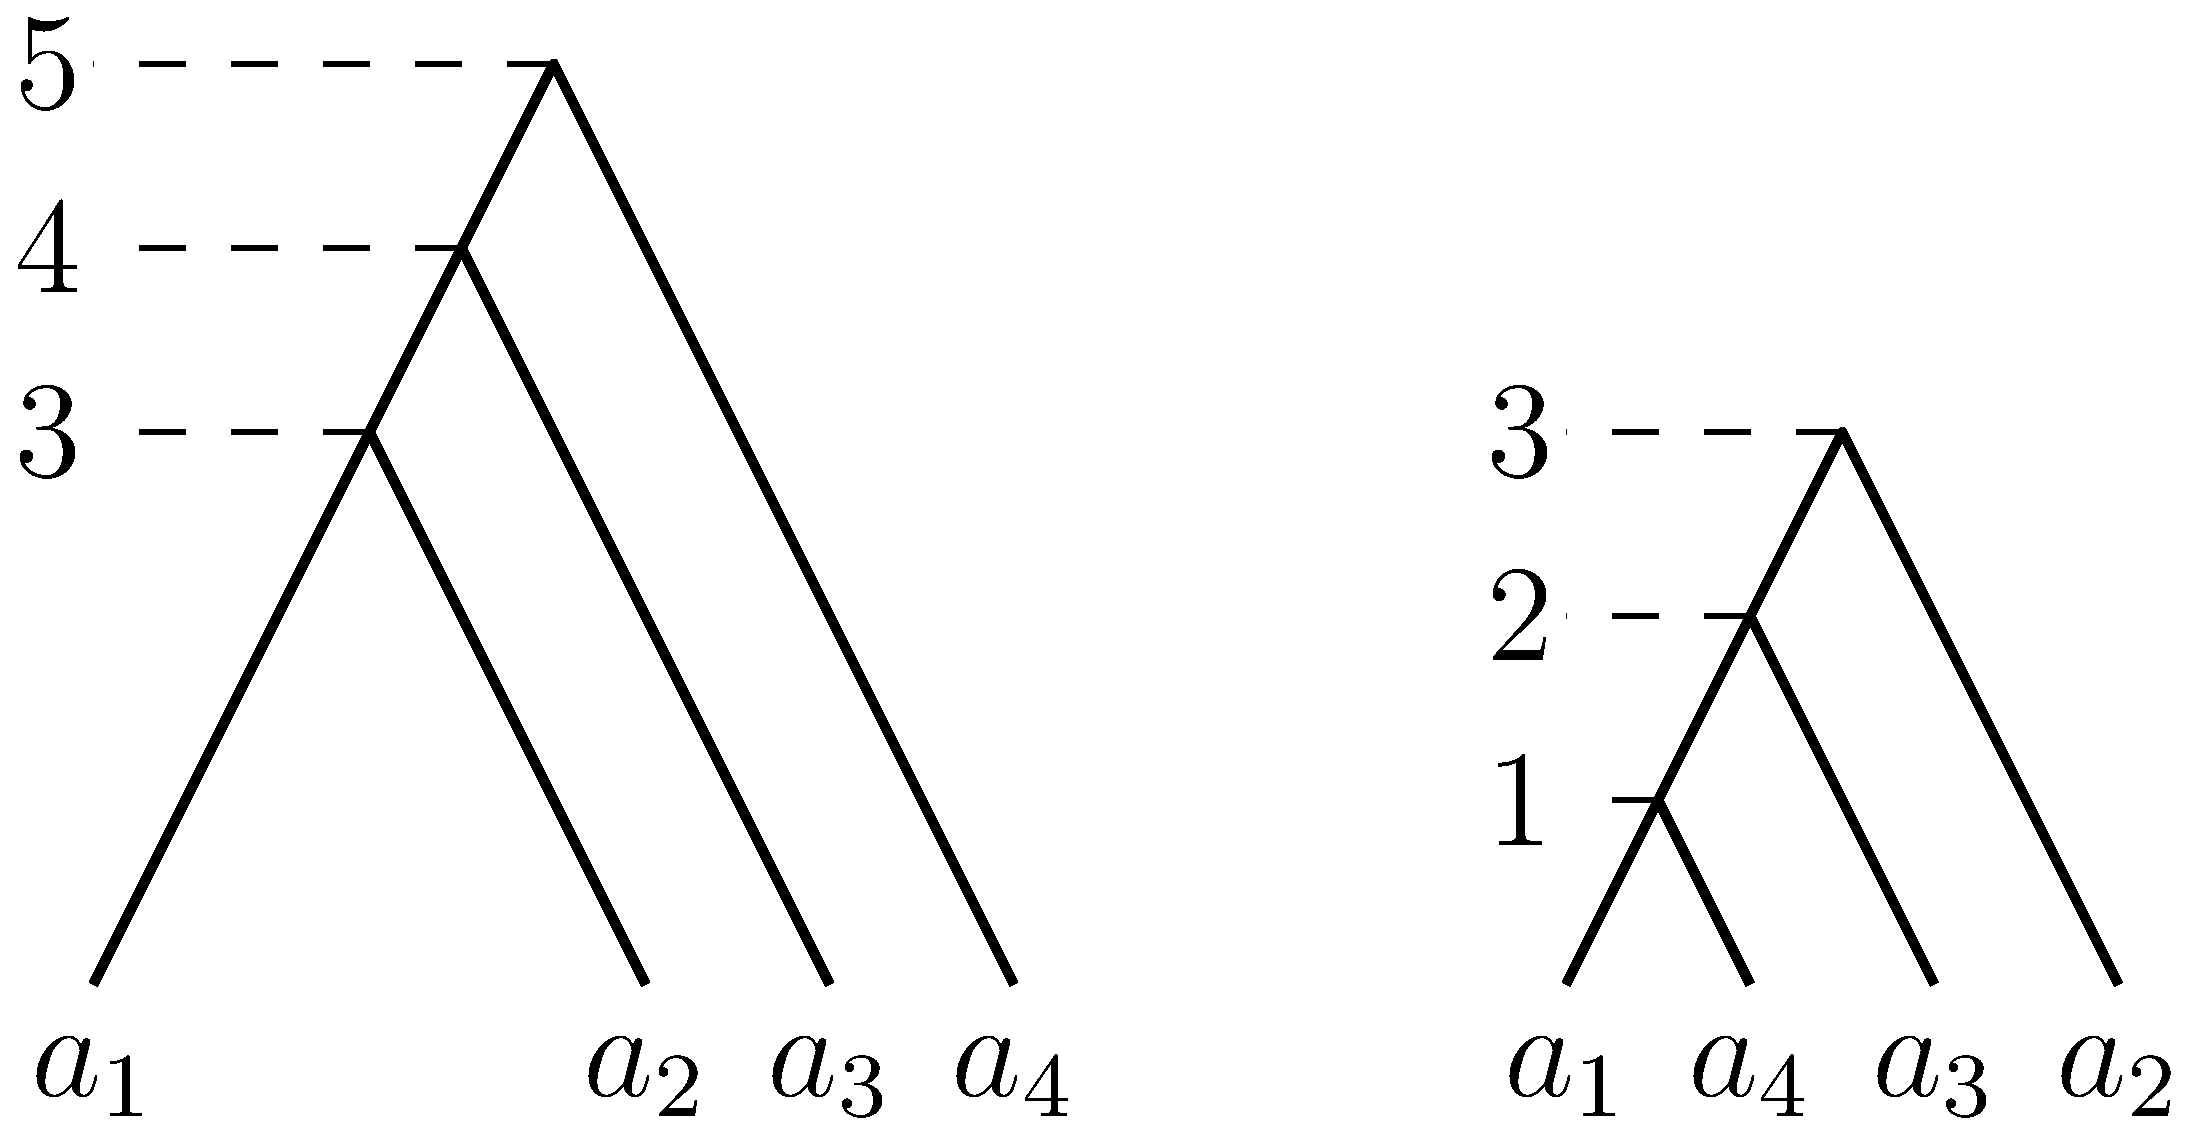
\includegraphics[width=0.65\textwidth]{cat_max_dist_dtt.eps}
		\caption{Trees with distance $m(n-1) - \frac{n(n-1)}{2}$}
		\label{fig:cat_max_dist_dtt}
	\end{figure}
\end{proof}

Note that the worst-case running time of $\findpath$ is $\O(n^2)$ and $\O(nm)$ in $\rnni$ and $\dtt_m$, respectively, and only depends on the diameter of the corresponding tree spaces.
For computing a shortest path, there is no algorithm with better worst-case running time than this, as the running time for algorithms computing shortest paths is bounded from below by the diameter of the corresponding space.

\summary{Radius of $\rnni$ is equal to its diameter.}
The \emph{radius} of a graph is defined as he minimum distance of any vertex in the graph to the vertex with maximum distance from it.
For $\dtt_m$ and $\rnni$, this is $\min\limits_{\text{tree } T}\max\limits_{\text{tree }R} d(T,R)$, where $d$ is a distance measure in the corresponding graph.
In the following we see that the radius of $\rnni$ equals its diameter, which we show to not be true for $\dtt_m$ afterwards.

\begin{lemma}
	The radius of $\rnni$ equals its diameter, that is $\frac{(n-1)(n-2)}{2}$.
	\label{lemma:radius_rnni}
\end{lemma}

\begin{proof}
	We prove this lemma by showing that every tree $T$ in $\rnni$ has a caterpillar tree $R$ with distance $\frac{(n-1)(n-2)}{2}$ to $T$.
	This will be proven by induction on the number of leaves $n$.

	The base case $n=3$ is trivial, as all three trees in this space are caterpillar trees with distance one from every other tree.
	For the induction step we consider an arbitrary tree $T$ with $n+1$ leaves.
	Let $x$ and $y$ be the leaves of $T$ that share the internal node of rank one as parent in $T$, and let $T'$ be the tree on $n$ leaves resulting from deleting one of these leaves, say $x$, of $T$.
	By the induction hypothesis there is a caterpillar tree $R'$ with distance $\frac{(n-1)(n-2)}{2}$ to $T'$.
	Now consider the tree $R$ resulting from adding $x$ at the top of $R'$ such that the root of $R$ has $x$ and $R'$ as children.

	We noe consider the path computed by $\findpath$ from $T$ to $R$.
	In the first iteration of $\findpath$, $(\{x,y\})_R$ moves down until it reaches rank one.
	Therefore, first $(x)_R$ moves down by $\nni$ moves until it reaches rank one more than $(y)_R$.
	Then a further $\nni$ move creates an internal node with children $x$ and $y$, before this node is moved down by rank swaps as depicted in Figure~\ref{fig:max_dist_ctree}.
	Altogether, there are $n-1$ $\rnni$ moves needed in the first iteration, as the rank of the parent of $x$ decreases by one within every move, starting at the root with rank $n$ and ending at the internal node of rank one.
	The tree at the end of this first iteration on $\fp(T,R)$ is identical to $R'$ when removing the leaf $x$ and suppressing its parent (the root, making the remaining child the new root).
	Since the cluster $\{x,y\}$ is not considered again in $\findpath$, the remaining part of $\fp(T,R)$ contains the same moves as $\fp(T',R')$, and hence $|\fp(T,R)| = |\fp(T',R')| + n-1$.
	Therefore it is $d(T,R) = \frac{(n-1)(n-2)}{2} + n-1 = \frac{n(n-1)}{2}$, which proves the lemma.
	\begin{figure}[ht]
		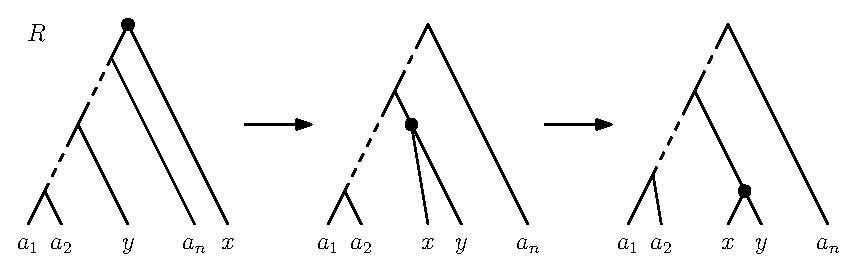
\includegraphics[width=0.8\textwidth]{max_dist_ctree.eps}
		\caption{Initial $n - 1$ $\rnni$ moves of $\fp(R,T)$ as described in the proof of Lemma~\ref{lemma:radius_rnni}.
		Removing the leaf $x$ and suppressing the non-root node of degree two from the tree on the right results in $R'$ as described in the lemma.}
		\label{fig:max_dist_ctree}
	\end{figure}
\end{proof}

Unlike in $\rnni$, the radius of $\dtt_m$ does not equal its diameter.
A counterexample is given by the tree depicted in \autoref{fig:dtt_radius_counterexample} on three leaves in $\dtt_4$.
There is no tree in $\dtt_4$ that has distance $m(n-1) - \frac{n(n-1)}{2}$ (diameter of $\dtt_m$) from that tree.

\begin{figure}[ht]
	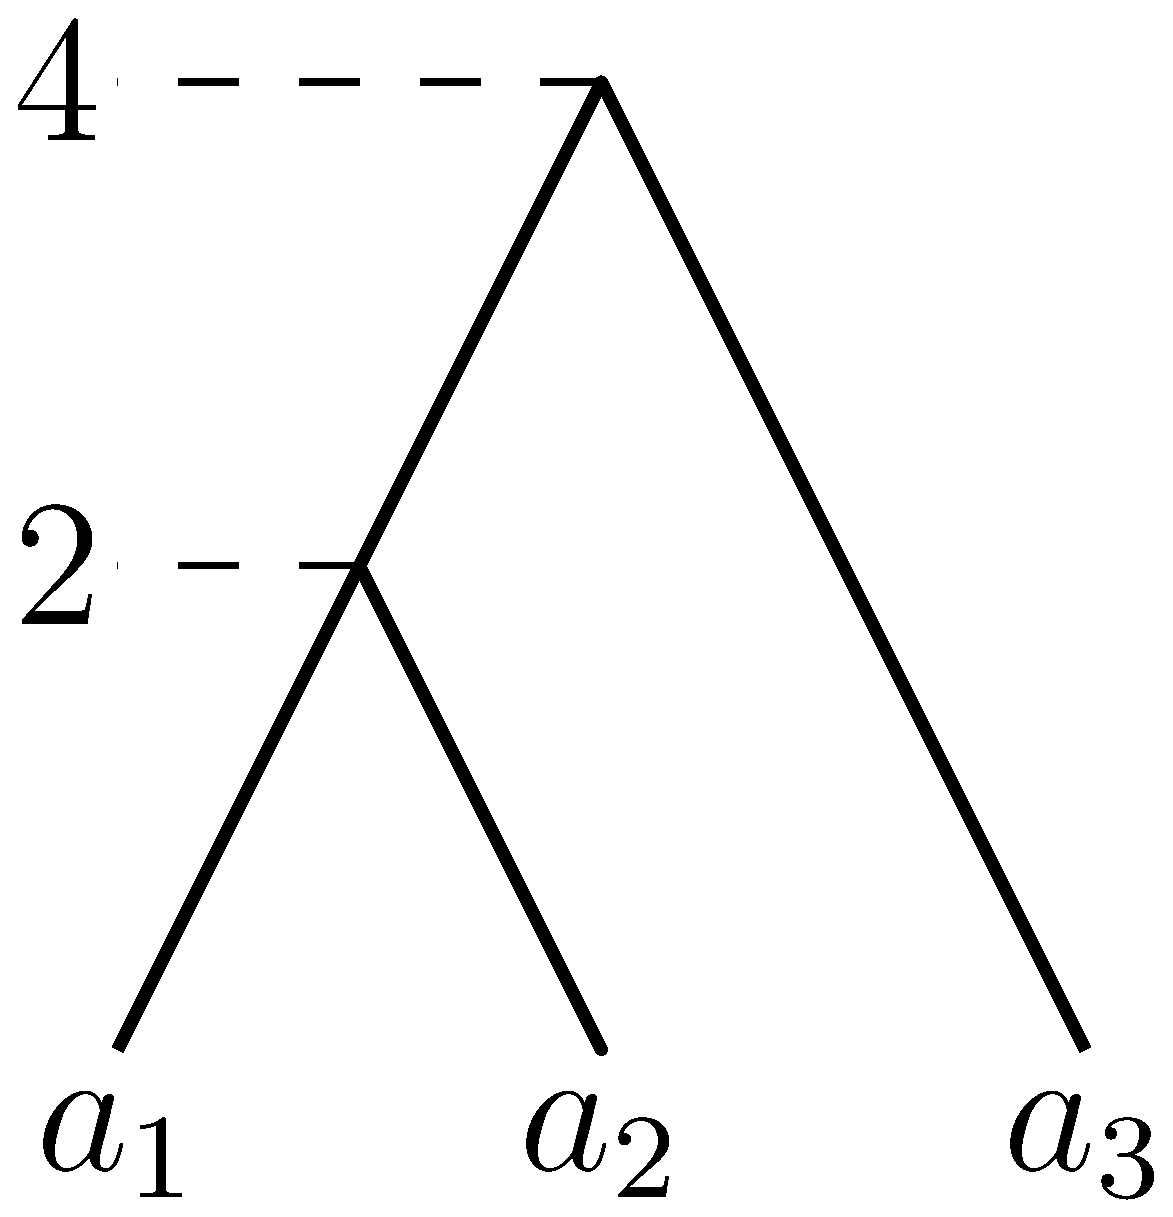
\includegraphics[width=0.15\textwidth]{dtt_radius_counterexample.eps}
	\caption{Tree in $\dtt_4$ on three leaves for which there is not tree with distance $5 = m(n-1) - \frac{n(n-1)}{2}$ (diameter) from it}
	\label{fig:dtt_radius_counterexample}
\end{figure}


\section{Discussion}

\summary{How partition lattices correspond to $\rnni$.}

\summary{Implementation of FP}

\subsection{Open Problems}

\summary{More efficient algorithm for computing distances (not shortest paths) -- mentioning David's results on mapping onto L1?}

\summary{Radius $\dtt_m$}

\summary{$\rnni(rho)$ and parameter $\rho$ for discrete time-trees}

\summary{scaling-free tree space}

\end{document}